\documentclass[11pt, a4paper]{article}

% --- UNIVERSAL PREAMBLE BLOCK FOR PDFLATEX ---
\usepackage[a4paper, top=1.5cm, bottom=2cm, left=1.5cm, right=1.5cm]{geometry}
\usepackage[T1]{fontenc}
\usepackage[utf8]{inputenc}
\usepackage[english]{babel}

% Set default font to Noto Sans (pdflatex compatible)
\usepackage[sfdefault]{noto-sans}

% Required packages
\usepackage{amsmath}
\usepackage{amssymb}
\usepackage{enumitem}
\usepackage{fancyhdr}
\usepackage{tikz}
\usetikzlibrary{patterns, calc}
\usepackage{booktabs}
\usepackage{calc}
\usepackage{graphicx}
\usepackage{xcolor}

% Define the specific colors for the logo
\definecolor{cometblue}{RGB}{0, 82, 155}
\definecolor{foundationgrey}{RGB}{120, 120, 120}

% Page styling
\pagestyle{fancy}
\fancyhf{}
\renewcommand{\headrulewidth}{0pt}
\fancyfoot[C]{\thepage}

\setlength{\parindent}{0pt}

\begin{document}

% --- HEADER SECTION ---
\begin{minipage}[c]{0.35\textwidth}
    
\begin{tikzpicture}[baseline=(base)]
        \node (base) at (0,0) {};
        \node[anchor=south west, cometblue, inner sep=0] (text) at (0, 0.4) {
            \fontsize{18}{18}\selectfont\textsf{{\bfseries IIITB COMET}}
        };
        \begin{scope}[shift={(text.south east)}, xshift=-0.25cm, yshift=0.75cm]
            \draw[line width=1.2pt, foundationgrey!50] (-0.4,0) arc (140:40:0.6);
            \draw[line width=1.2pt, foundationgrey!75] (-0.55,0.15) arc (140:40:0.8);
            \draw[line width=1.2pt, foundationgrey] (-0.7,0.3) arc (140:40:1.0);
        \end{scope}
        \node[anchor=north west, foundationgrey, inner sep=0] at (0, 0.35) {
            \fontsize{8.5}{8.5}\selectfont\textsf{{\bfseries \makebox[\widthof{\fontsize{18}{18}\selectfont\textsf{{\bfseries IIITB COMET}}}][s]{F O U N D A T I O N}}}
        };
    \end{tikzpicture}
\end{minipage}
\hfill
\begin{minipage}[c]{0.35\textwidth}
    \centering
    {\huge {\bfseries MATHEMATICS}} \\
    \vspace{0.1cm}
    {\small Time allowed: $3$ hours \quad | \quad Max Marks: $80$}
\end{minipage}
\hfill
\begin{minipage}[c]{0.28\textwidth}
    \raggedleft
    \footnotesize
    {\bfseries Name:} Jera Prakash \\
    {\bfseries ID:} COMETFWC38 \\
    {\bfseries Date:} $22$ January $2026$ \\
    {\bfseries Code No. 30/1}
\end{minipage}

\vspace{0.8em}
\hrule[1pt]
\vspace{1em}

\section*{General Instructions}
\begin{enumerate}[label=\arabic*., nosep]
    \item All questions are compulsory.
    \item The question paper consists of $31$ questions divided into four sections --- A, B, C and D.
    \item Section A contains questions $1$ to $4$ ($1$ mark each).
    \item Section B contains questions $5$ to $10$ ($2$ marks each).
    \item Section C contains questions $11$ to $22$ ($3$ marks each).
    \item Section D contains questions $23$ to $31$ ($4$ marks each).
\end{enumerate}

\vspace{1em}
\hrule
\vspace{1em}

\section*{SECTION A}

\begin{enumerate}[label=\arabic*.]
    \item If $x=3$ is one root of the quadratic equation $x^2 - 2kx - 6 = 0$, then find the value of $k$.
    \item What is the HCF of the smallest prime number and the smallest composite number?
    \item Find the distance of a point $P(x, y)$ from the origin.
    \item In an AP, if the common difference $d = -4$, and the seventh term $a_7$ is $4$, then find the first term $a$.
\end{enumerate}

\section*{SECTION B}

\begin{enumerate}[label=\arabic*., resume]
    \item Find the ratio in which $P(4, m)$ divides the line segment joining the points $A(2, 3)$ and $B(6, -3)$. Hence find $m$.
    \item Two different dice are tossed together. Find the probability: \\
    (i) of getting a doublet \hspace{1cm} (ii) of getting a sum $10$, of the numbers on the two dice.
    \item An integer is chosen between $70$ and $100$. Find the probability that it is: \\
    (a) a prime number \hspace{3cm} (b) divisible by $7$
    \item Solve for $x$: $\sqrt{3}x^2 + 10x + 7\sqrt{3} = 0$.
    \item Find the number of natural numbers between $101$ and $999$ which are divisible by both $2$ and $5$.
    \item A statue $1.6$ m tall stands on the top of a pedestal. From a point on the ground, the angle of elevation of the top of the statue is $60^\circ$ and from the same point the angle of elevation of the top of the pedestal is $45^\circ$. Find the height of the pedestal.
    
    \begin{center}
    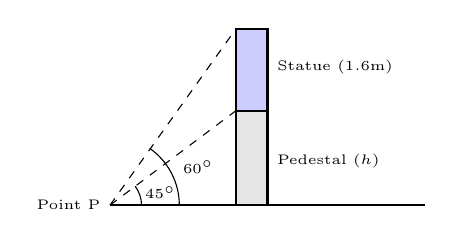
\begin{tikzpicture}[scale=0.8]
        \draw[thick] (0,0) -- (5,0); % Ground
        \draw[thick, fill=gray!20] (2,0) rectangle (2.5,1.5); % Pedestal
        \draw[thick, fill=blue!20] (2,1.5) rectangle (2.5,2.8); % Statue
        \node[right, font=\tiny] at (2.5, 2.2) {Statue ($1.6$m)};
        \node[right, font=\tiny] at (2.5, 0.7) {Pedestal ($h$)};
        \draw[dashed] (0,0) -- (2,1.5);
        \draw[dashed] (0,0) -- (2,2.8);
        \node[left, font=\tiny] at (0,0) {Point P};
        \draw (0.5,0) arc (0:37:0.5);
        \node at (0.8,0.2) {\tiny $45^\circ$};
        \draw (1.1,0) arc (0:55:1.1);
        \node at (1.4,0.6) {\tiny $60^\circ$};
    \end{tikzpicture}
    \end{center}
\end{enumerate}

\section*{SECTION C}

\begin{enumerate}[label=\arabic*., resume]
    \item Use Euclid's division algorithm to find the HCF of $4052$ and $12576$.
    \item Find the zeroes of the quadratic polynomial $6x^2 - 3 - 7x$ and verify the relationship between the zeroes and the coefficients.
    \item Solve the following pair of linear equations: $3x + 4y = 10$ and $2x - 2y = 2$.
    \item Evaluate: $\int (x+3)\sqrt{3-4x-x^{2}}\,dx$.
    \item Find the particular solution of the differential equation $\frac{dy}{dx} = -\frac{x+y \cos x}{1+\sin x}$ given that $y(0)=1$.
    \item Find the particular solution of $2ye^{x/y}dx + (y-2xe^{x/y})dy = 0$, given $x=0$ when $y=1$.
    \item Show that the points $A(4, 5, 1)$, $B(0, -1, -1)$, $C(3, 9, 4)$, and $D(-4, 4, 4)$ are coplanar.
    \item Find the foot of the perpendicular from $A(-1, 8, 4)$ to the line joining $B(0, -1, 3)$ and $C(2, -3, -1)$. Hence find the image of point $A$ in line $BC$.
    \item Three numbers are chosen at random from the first six positive integers. Let $X$ be the largest number. Find the probability distribution of $X$.
    \item Let $A = \mathbb{R} \times \mathbb{R}$ and define $(a, b) * (c, d) = (a + c, b + d)$. Show that $*$ is commutative and associative.
    \item Prove that $y = \frac{4 \sin \theta}{2 + \cos \theta} - \theta$ is increasing on $[0, \pi/2]$.
\end{enumerate}

\section*{SECTION D}

\begin{enumerate}[label=\arabic*., resume]
    \item Using integration, find the area of the triangle with vertices $(2, 2)$, $(4, 3)$, and $(1, 2)$.
    \item Find the equation of the plane containing the line of intersection of the planes $\vec{r} \cdot (\hat{i} + \hat{j} + \hat{k}) = 1$ and $\vec{r} \cdot (2\hat{i} + 3\hat{j} - \hat{k}) + 4 = 0$ and which is perpendicular to the plane $\vec{r} \cdot (\hat{i} - \hat{j} + \hat{k}) = 0$.
    \item Prove that the angle between the two tangents drawn from an external point to a circle is supplementary to the angle subtended by the line-segment joining the points of contact at the centre.
    
    \begin{center}
    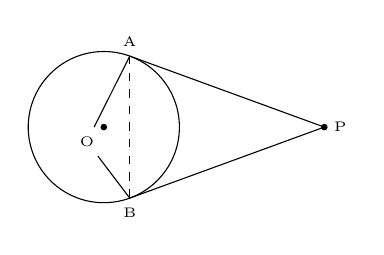
\begin{tikzpicture}[scale=0.8]
        \draw (0,0) circle (1.2);
        \node (O) at (0,0) [below left, font=\tiny] {O};
        \fill (0,0) circle (1.5pt);
        \coordinate (P) at (3.5,0);
        \fill (P) circle (1.5pt) node[right, font=\tiny] {P};
        \coordinate (A) at ({1.2*1.2/3.5}, {1.2*sqrt(1-(1.2/3.5)^2)});
        \coordinate (B) at ({1.2*1.2/3.5}, {-1.2*sqrt(1-(1.2/3.5)^2)});
        \draw (P) -- (A) node[above, font=\tiny] {A};
        \draw (P) -- (B) node[below, font=\tiny] {B};
        \draw (O) -- (A);
        \draw (O) -- (B);
        \draw[dashed] (A) -- (B);
    \end{tikzpicture}
    \end{center}

    \item The sum of the first three terms of an AP is $33$. If the product of the first and the third term exceeds the second term by $29$, find the AP.
    \item A hemispherical tank full of water is emptied by a pipe at the rate of $3\frac{4}{7}$ litres per second. How much time will it take to empty half the tank, if it is $3$ m in diameter?
    \item If $\sec\theta + \tan\theta = p$, then find the values of $\sin\theta$ and $\cos\theta$ in terms of $p$.
    \item A bucket is in the form of a frustum of a cone with a capacity of $12308.8$ cm$^3$. The radii of the top and bottom circular ends are $20$ cm and $12$ cm respectively. Find the height of the bucket and its surface area. (Use $\pi = 3.14$)
    \item If the median of the distribution given below is $28.5$, find the values of $x$ and $y$.
    
    \begin{center}
    \small
    \begin{tabular}{|c|c|c|c|c|c|c|c|}
    \hline
    {\bfseries Class interval} & $0-10$ & $10-20$ & $20-30$ & $30-40$ & $40-50$ & $50-60$ & {\bfseries Total} \\ \hline
    {\bfseries Frequency} & $5$ & $x$ & $20$ & $15$ & $y$ & $5$ & {\bfseries 60} \\ \hline
    \end{tabular}
    \end{center}

    \item Prove that the ratio of the areas of two similar triangles is equal to the square of the ratio of their corresponding sides.
\end{enumerate}

\end{document}
